\section{سوال اول}
\subsection{موشک هوا به زمین}
برای این بخش موشک هوا به زمین
\lr{AGM-158 JASSM\LTRfootnote{Joint Air-to-Surface Standoff Missile}}
در نظر گرفته شده است. شکل آن در پایین آورده شده است.
 \begin{figure}[H]
	\centering
	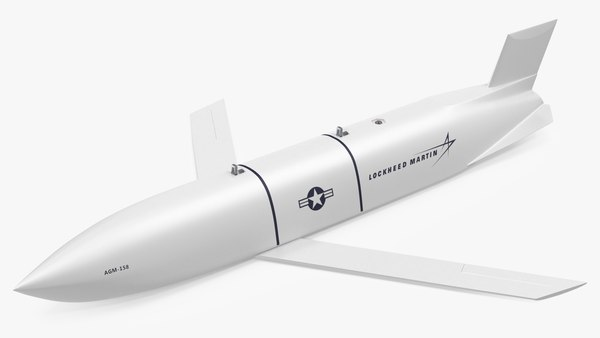
\includegraphics[width=\linewidth]{../Figure/Q1/agm_158.jpg}
	\caption{موشک هوا به زمین
\lr{AGM-158}	
}
\end{figure}
\subsubsection{اجزای سیستم هدایت}
\begin{itemize}
	\item حسگرهای هدایت
	این موشک حسگرهای هدایت متنوعی برای فازهای مختلف هدایت دارد. این حسگرها شامل سیستم ناوبری اینرسی\LTRfootnote{Inertial Navigation System}
	 همراه با سیستم موقعیت یابی جهانی زد پارازیت\LTRfootnote{Anti-Jam Global Positioning System}
	 و ژیروسکوپ لیزری\LTRfootnote{Ring Laser Gyro Inertial Measurement Unit}
	 است. سایر حسگرهای هدایت شامل جستجوگر تصویربرداری مادون قرمز\LTRfootnote{Imaging Infrared (I2R) Seeker}
	و همبسته هدف خودکار\LTRfootnote{Automatic Target Correlator}
	برای نرخ برخورد با دقت بالا است.
	\item پردازنده هدایت
	با توجه به ماموریت و برد بلند آن که امکان پارازیت است، پردازنده آن داخلی است.
	\item الگوریتم هدایت
	با توجه به اینکه مسیر طولانی‌ای را طی می‌کند مسیر پروازی از نوع کروز یا بهینه است. از طرفی، با توجه به مسیر، حسگر و کامپیوتر پرواز، برای دقت بالاتر، الگوریتم هدایت حلقه بسته است.
	\item تجهیزات مخابراتی
	برای این پرنده فرمان کنترلی ارسال نمی‌شود. اما پرنده می‌تواند وضعیت خود، تصویر دوربین و زمان برخورد را جهت بررسی عملکرد پرنده به اپراتور ارسال کند.
\end{itemize}
\subsubsection{مراحل هدایت و هدف}
مراحل هدایت این وسیله پرنده، شامل سه فاز آغازین (پرتاب)، میانی و پایانی است که هر کدام به اختصار بیان شده است.
\begin{itemize}
	\item فاز پرتاب
	فاز پرتاب را می‌توان به صورت حلقه باز در نظر گرفت. در این فاز هدف دور شدن از پرنده و رسیدن به سرعت کنترلی است. 
	این فاز نیاز به محاسبات زیادی ندارد و می‌توان فرمان‌ها را به صورت تابعی از زمان اجرا کرد.
	 \begin{figure}[H]
		\centering
		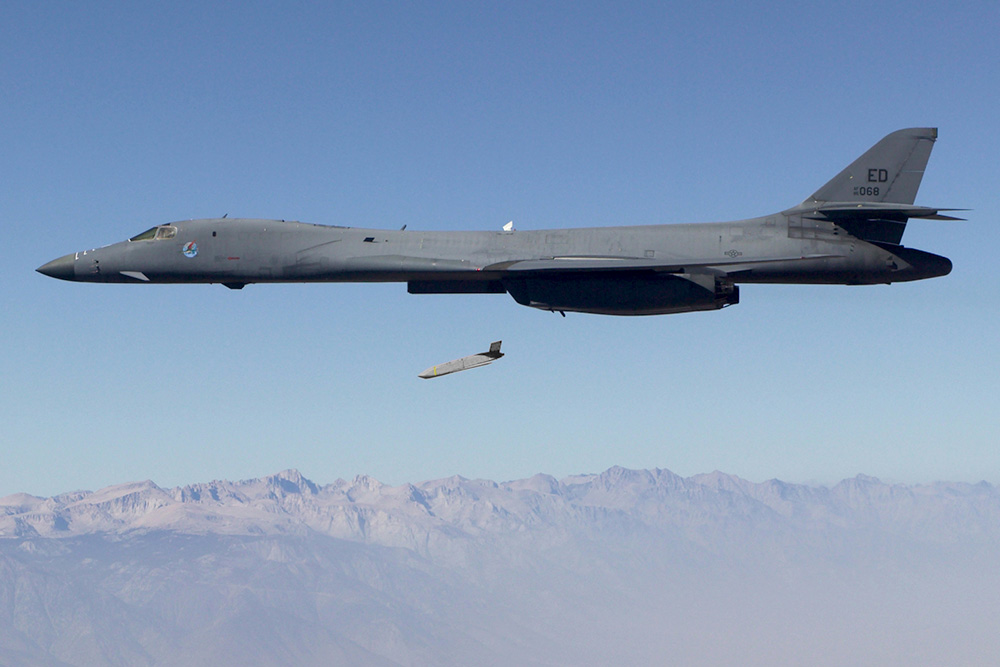
\includegraphics[width=\linewidth]{../Figure/Q1/start.jpg}
		\caption{فاز پرتاب موشک هوا به زمین
			\lr{AGM-158}	
		}
	\end{figure}
	
	\item فاز میانی
	به دلیل اینکه فاز میانی کروز و طولانی است نیاز به دریافت اطلاعات موقعیت به صورت دقیق و لحظه‌ای است تا مسیر بهینه‌ای را طی کند. بنابراین، حلقه بسته است. در این فاز، هدف نزدیک شدن به هدف با کمترین انرژی و بیشترین دقت است.
		 \begin{figure}[H]
		\centering
		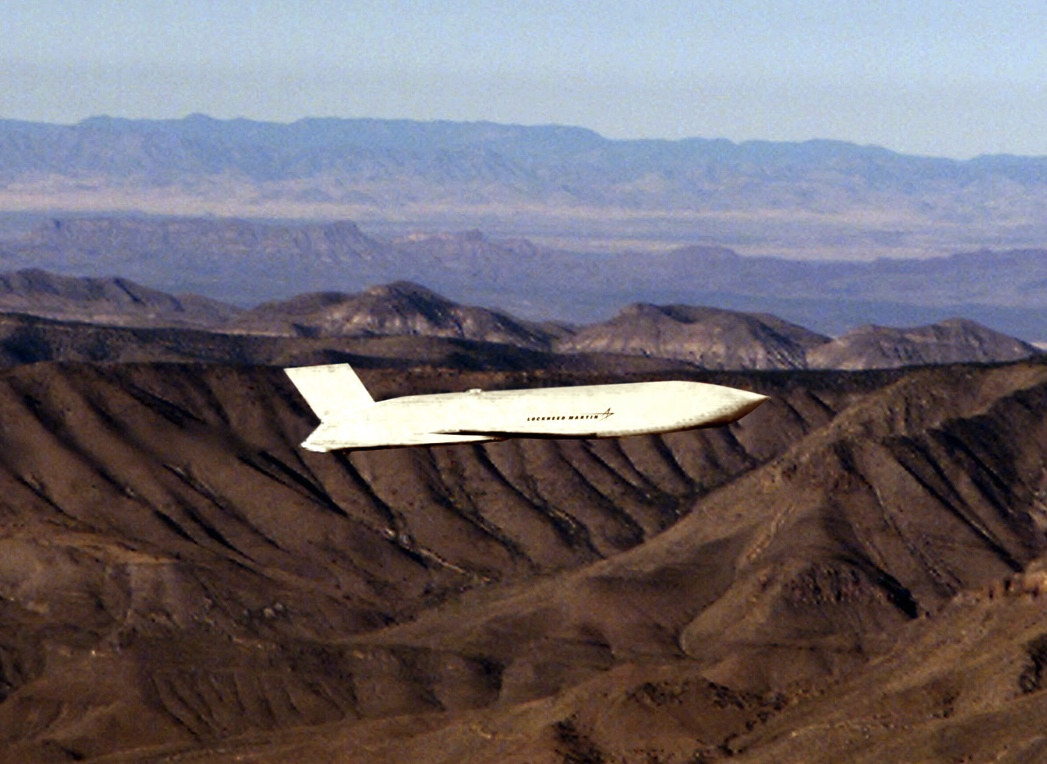
\includegraphics[width=\linewidth]{../Figure/Q1/cruise.jpg}
		\caption{فاز میانی موشک هوا به زمین
			\lr{AGM-158}	
		}
	\end{figure}

	\item فاز پایانی
	با توجه به اینکه دقت این موشک بالا است، نیاز دارد در هر لحظه بر اساس وضعیت تصمیم بگیرد. بنابراین، این فاز هم به صورت حلقه بسته است. هدف در این فاز، برخورد دقیق به هدف است.
			 \begin{figure}[H]
		\centering
		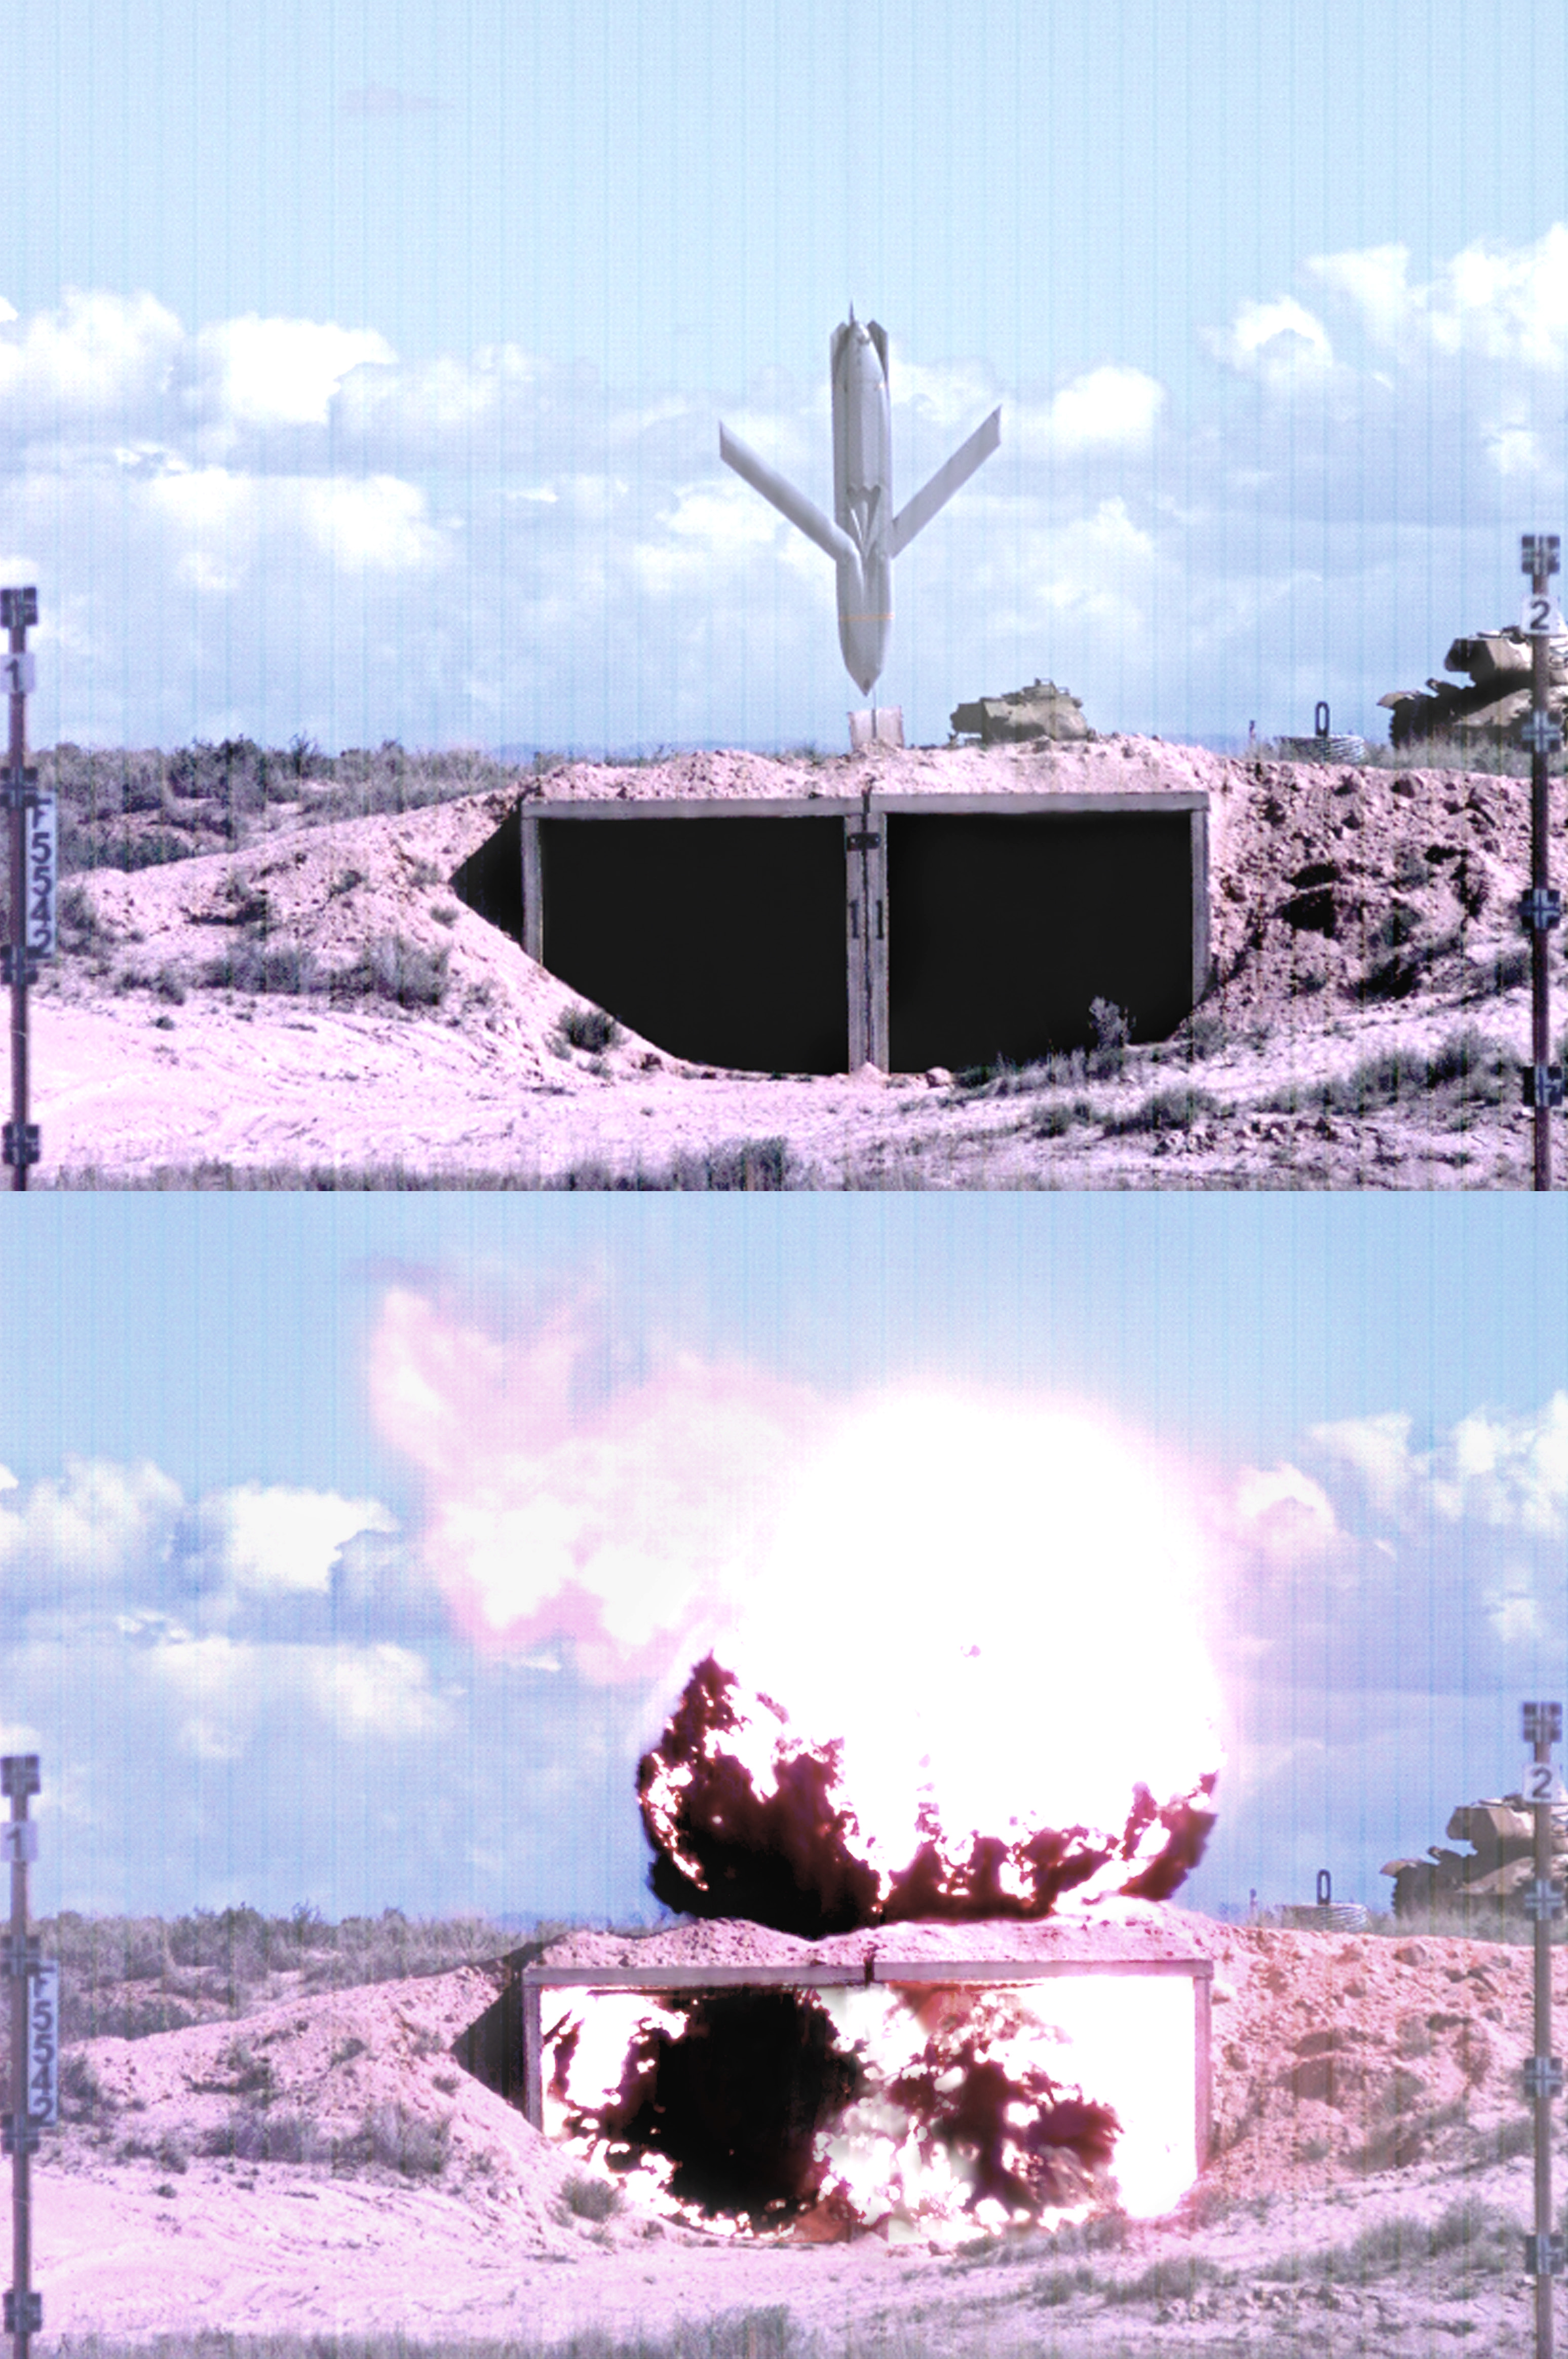
\includegraphics[width=0.75\linewidth]{../Figure/Q1/end.jpg}
		\caption{فاز پایانی موشک هوا به زمین
			\lr{AGM-158}	
		}
	\end{figure}
\end{itemize}

\subsubsection{انتخاب مسیر هدایت}

در فاز اولیه به دلیل اینکه هدف صرفا دور شدن از پرنده است، مسیر هدایت خاصی را طی نمی‌کند و صرفا مسیر مستقیم را طی می‌کند. برای فاز میانی سه حالت بهینه و مبتنی بر عوارض زمین در نظر گرفت. از طرفی می‌توان برای فاز میانی دو نوع مسیر را در نظر گرفت. به این صورت که، ابتدای مسیر به صورت بهینه پرواز کند و در انتها مبتنی بر عوارض زمین. با این انتخاب مسیر، در ابتدا سوخت کمتری مصرف می‌شود و در انتها چون در داخل منطقه دشمن است، ناشناس بماند. در فاز پایانی، به دلیل داشتن جستجوگر به صورت مسیر خط دید در نظر گرفته شده است.
\subsubsection{نوع حسگرهای هدایت}
بر اساس توضیحات ارائه شده دارای حسگر مطلق و نسبی است. آشکارساز ندارد و سیستم ردگیری به‌صورت غیرفعال است.
خروجی حسگرها شامل موقعیت در دستگاه اینرسی، نرخ ژیروسکوپ،  زاویه دید هدف و نرخ چرخش خط دید نسبت به فضای اینرسی است.
\subsubsection{سیستم ناوبری}
در فاز میانی از ناوبری ترکیبی اینرسی و رادیویی استفاده شده است. در فاز پایانی هم اگر هدف به صورت موقعیت باشد، می‌توان مانند بخش قبل عمل کرد. در فاز پایانی ممکن است از جستجوگر استفاده شود.
\subsubsection{سیستم هدایت}
در فاز میانی از سیستم هدایت اینرسی، و در انتها از سیستم هدایت ترکیبی  اینرسی و آشیانه‌یاب استفاده شده است.
